\chapter{\tool ---补丁定位方法}

本章将详细阐述\tool ---一种基于多源知识的开源软件漏洞的补丁识别方法的设计。

\section{方法概述}
\begin{figure*}[h]
    \centering
    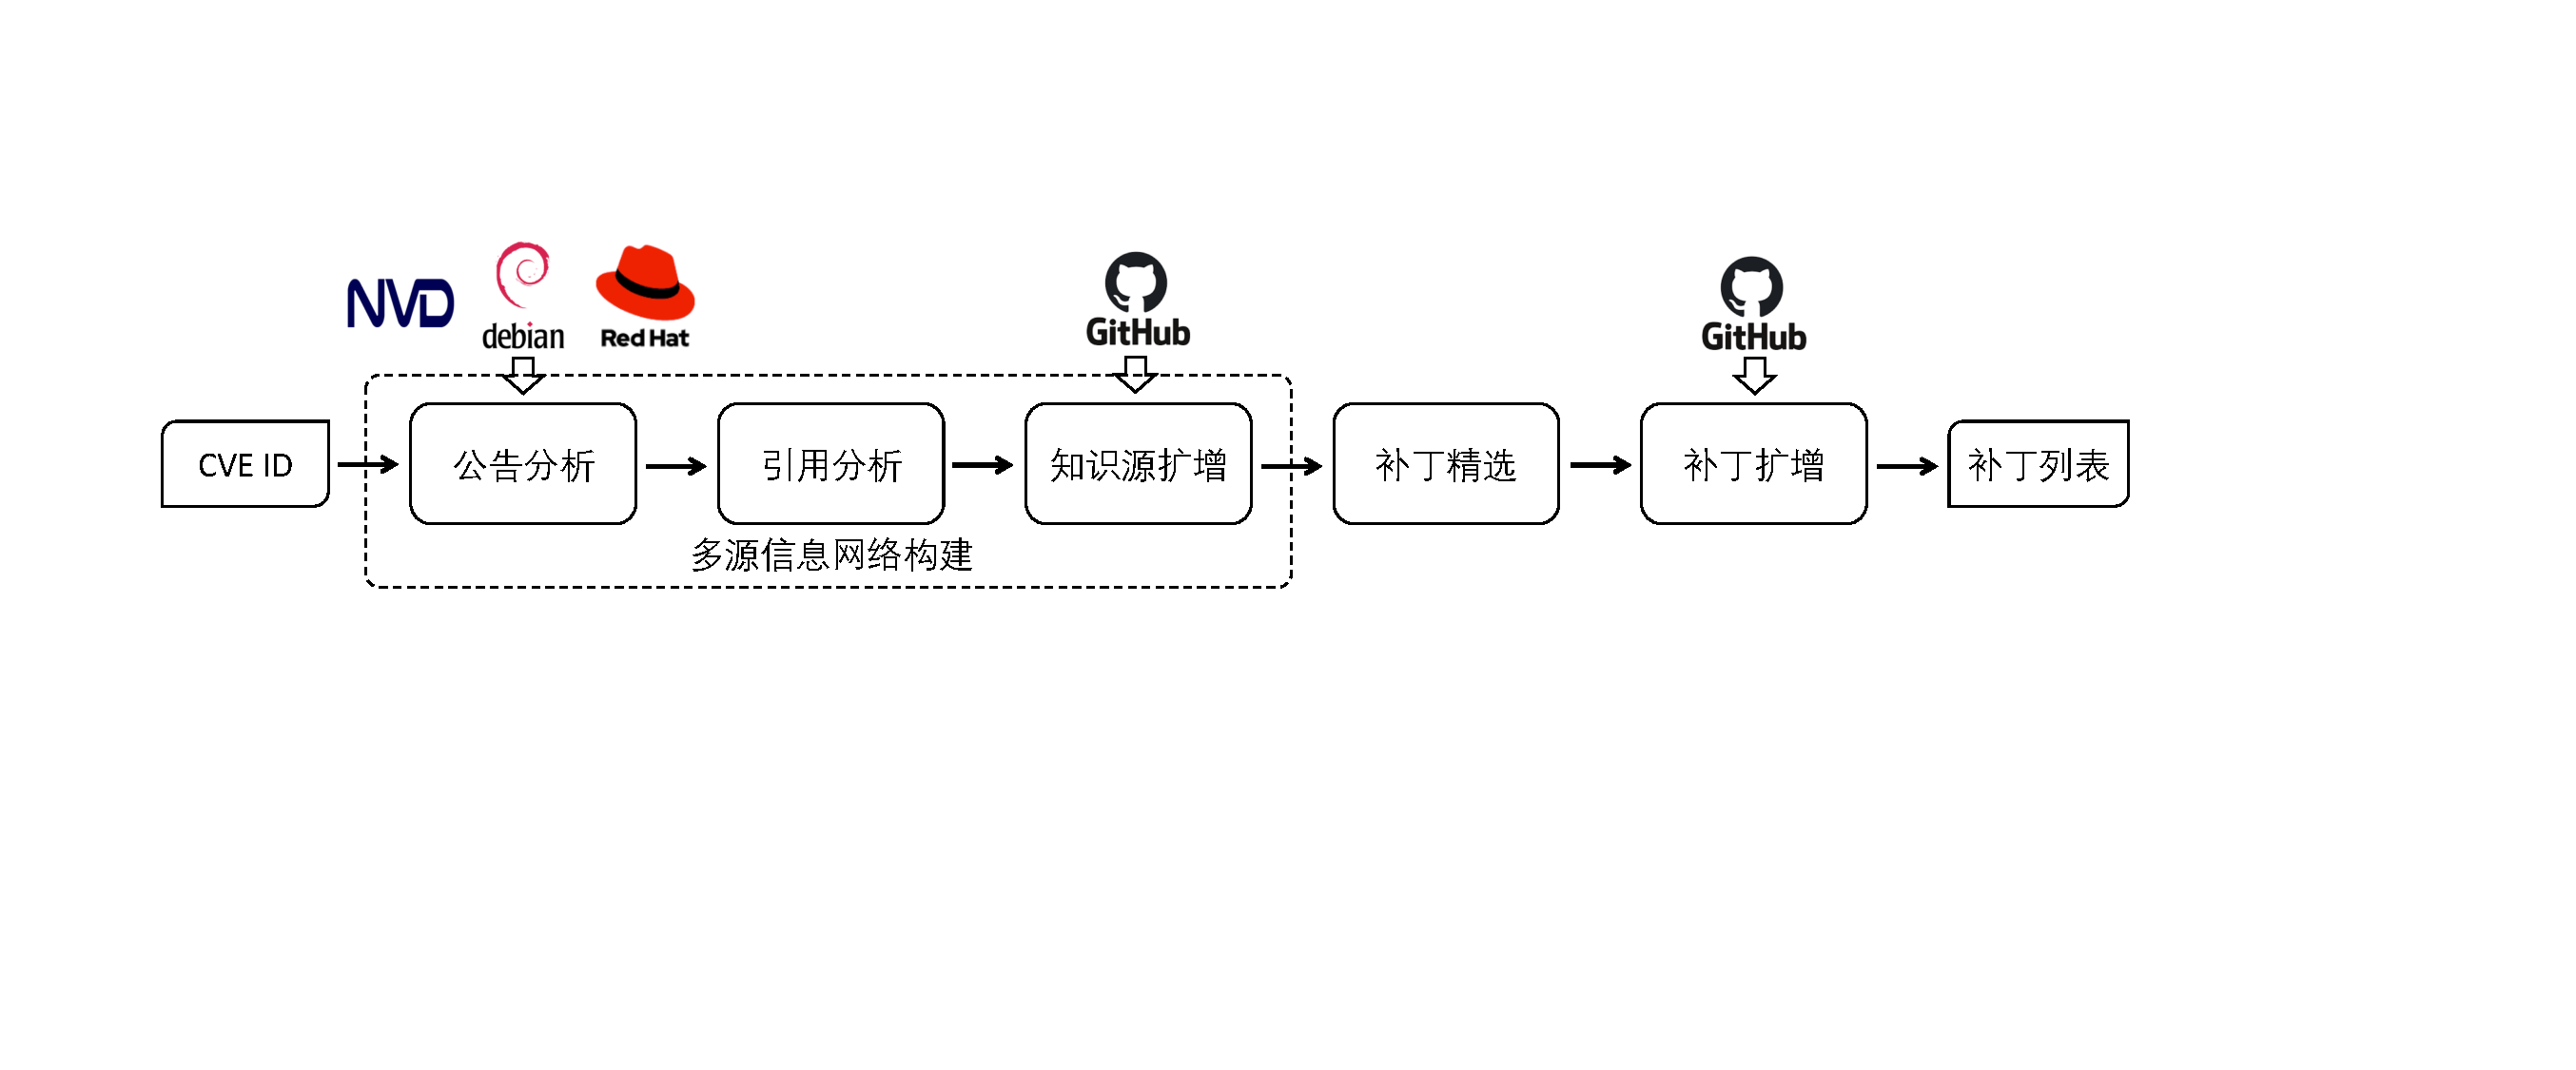
\includegraphics[scale=0.40]{res/overview.pdf}
    %\vspace{-10pt}
    \caption{\tool 方法概览}\label{fig:overview}
\end{figure*}

基于上文经验研究的发现,本文提出了一种名为\tool 的自动化方法来查找来源软件漏洞的补丁(Github Commit形式)。\tool 的基本思想是:漏洞的补丁信息(即:commit)会在与该漏洞相关的各种来源的漏洞公告、分析报告、讨论和解决的过程中被频繁提及和引用。

图\ref{fig:overview}展示了\tool 的方法概览。\tool 以漏洞的CVE标识符作为输入,最终返回其补丁信息。具体分为三步:首先,\tool 从多个\tocheck{信息源}(即:NVD、Debian\cite{debian}、RedHat\cite{redhat}和GitHub)为输入的CVE构建一个相关引用链接的信息网络。该步骤的目的是将CVE在报告、讨论和解决阶段的引用链接信息进行建模。这里将NVD视为主信息来源,将Debian、RedHat和GitHub视为次级信息来源,该级信息源可以进一步扩展。其次,\tool 从构建的参考链接网络中,选择中具有高连通性和高置信度的补丁节点(即:commit)作为该CVE的补丁。最后,\tool 通过搜索同一存储库中其他分支上的相关提交来扩展补丁集。该步骤目的是在CVE及其补丁之间建立潜在的一对多映射关系。在本章的其他小节中,将详细阐述每个步骤。

% \begin{itemize}[leftmargin=*]
% \item 首先,\tool 从多个\tocheck{信息源}(即:NVD、Debian\cite{debian}、RedHat\cite{redhat}和GitHub)为输入的CVE构建一个相关参考链接的网络。该步骤的目的是将CVE在报告、讨论和解决阶段的参考链接信息进行建模。这里将NVD视为主信息来源,将Debian、RedHat和GitHub视为次级信息来源,该级信息源可以进一步扩展。
% \item 其次,\tool 从构建的参考链接网络中,选择中具有高连通性和高置信度的补丁节点(即:commit)作为该CVE的补丁。
% \item 最后,\tool 通过搜索同一存储库中其他分支上的相关提交来扩展补丁集。该步骤目的是在CVE及其补丁之间建立潜在的一对多映射关系。
% \end{itemize}

\section{步骤一:构建多源引用信息网络}
\tool 的步骤一共包括三个子步骤,前两个子步骤为漏洞公告分析和引用分析,通过分析来自NVD、Debian和Red Hat三个信息源的漏洞公告构建初始引用信息网络;第三个子步骤为信息增强,通过从GitHub搜索相关提交链接来扩充信息网络。

\subsection{公告节点分析} \label{sec:advisory analysis}
首先,\tool 初始化信息网络,将输入的CVE-ID设置为根节点,然后再添加三个漏洞公告源节点(即:NVD、Debian和Red Hat)作为root的子节点。这些公告源节点用于追溯最终选定的补丁节点的来源。

\begin{figure}[h]
    \centering
    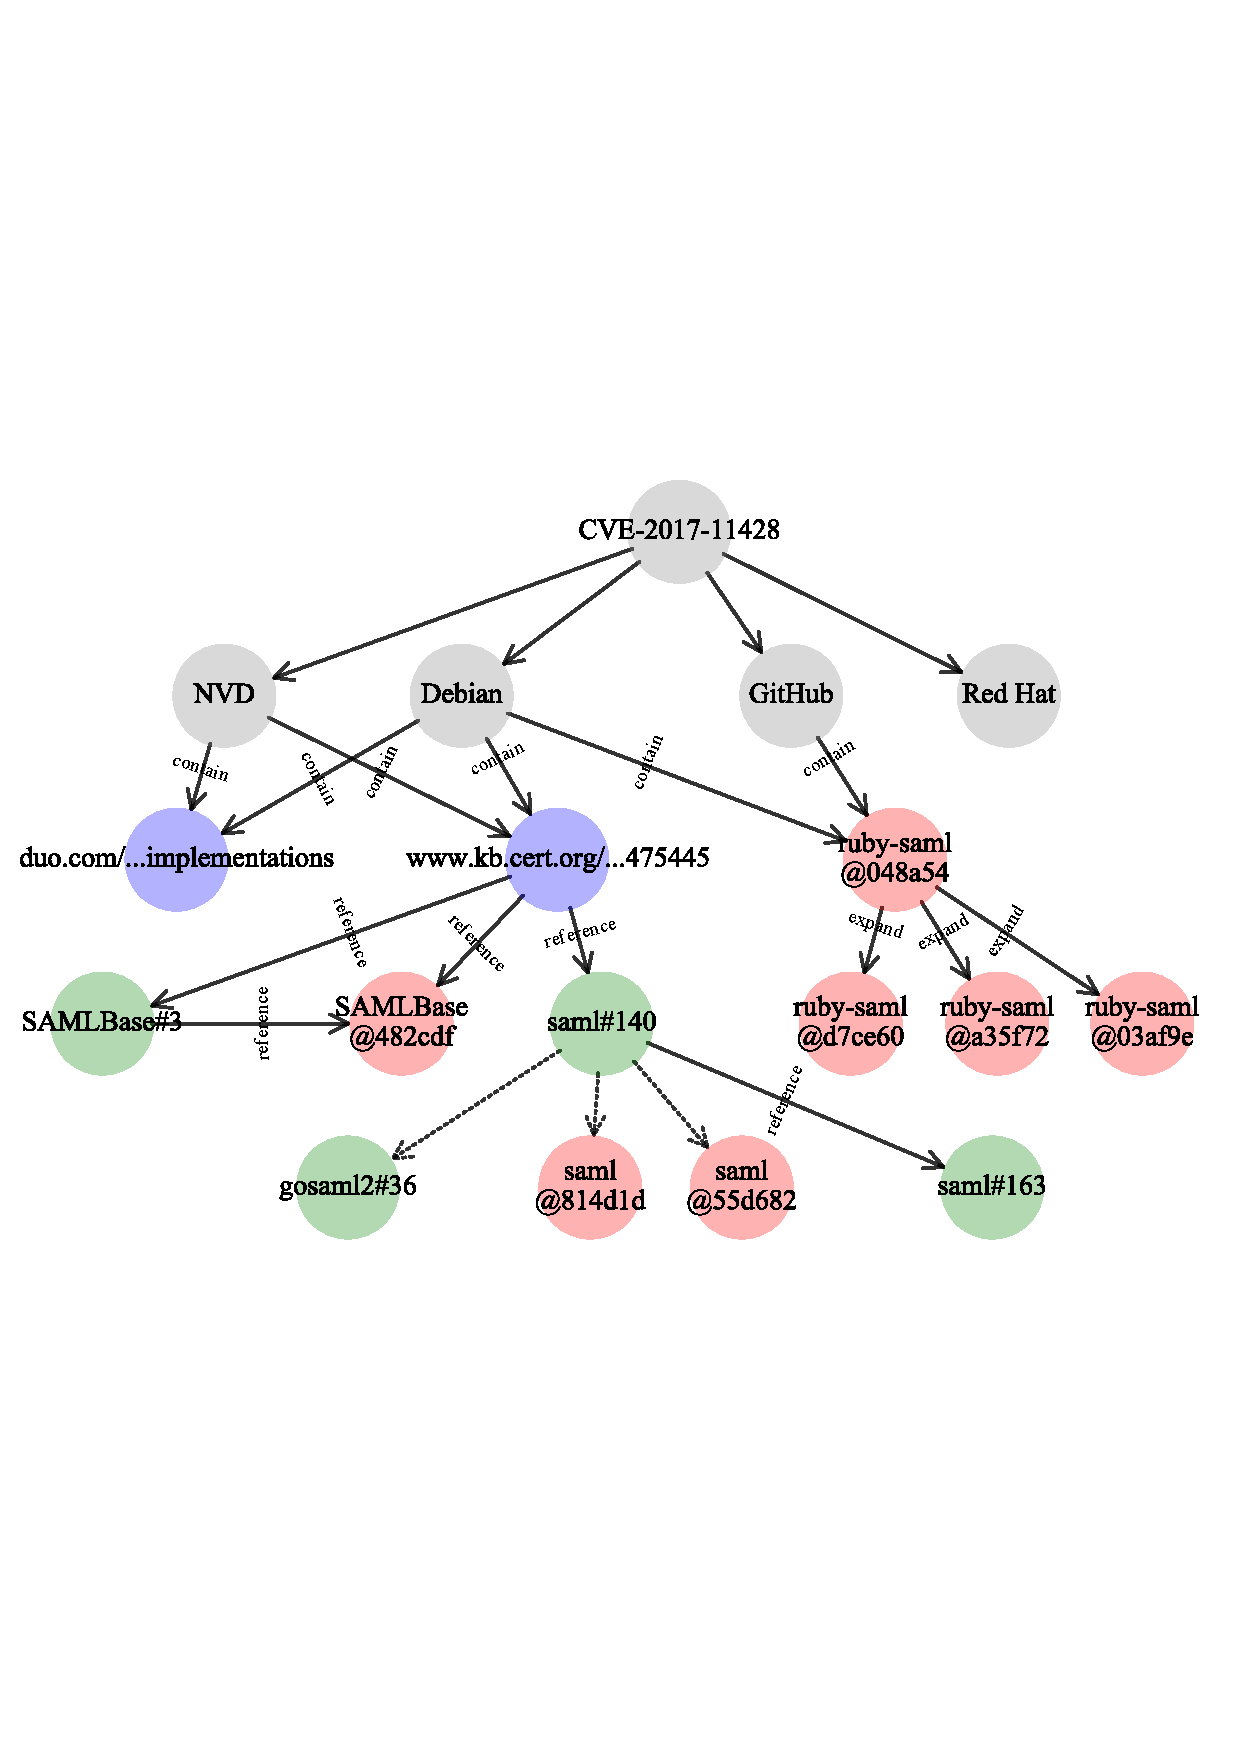
\includegraphics[scale=0.68]{res/network-example.pdf}
    %\vspace{-10pt}
    \caption{样例CVE-2017-11428的多源信息网络}\label{fig:example}
\end{figure}

\begin{exmp}
图\ref{fig:example}为样例CVE-2017-11428的完整的多源引用信息网络。 其中,顶层显示根节点,第二层显示公告来源节点。
\end{exmp}

然后,\tool 基于CVE-ID分别获取NVD、Debian和Red Hat的漏洞公告。其中,NVD平台以JSON形式按年份提供所有漏洞的结构化数据\cite{nvd-feed},\tool 通过下载并解析相应的JSON文件即可获得NVD中该CVE的信息。Debian平台的漏洞公告存储在仓库\cite{debian-repo}中,\tool 可直接从中解析得Debian提供的该CVE。Red Hat平台提供了 WebService API\cite{redhat-api}服务,\tool 可以直接使用该服务来检索Red Hat平台的漏洞公告。值得注意的是,分析发现:Debian会跟踪NVD上的所有CVE漏洞,而Red Hat仅会跟踪部分CVE漏洞。

\tool 从每个信息源的漏洞公告中提取引用信息(即:URL),并将它们添加为相应公告源节点的子节点。对于NVD公告,\tool 从“references”字段中提取出相关URL;类似地,对于Debian公告,\tool 会从“Notes”字段中提取出相关URL;对于Red Hat公告,\tool 使用正则表达式从评论区“comments”字段中提取出相关URL,这是因为开发人员会在评论区讨论和记录漏洞的解决过程,并可能列出对补丁信息。

\begin{exmp}
如图\ref{fig:example}中的第三层所示,对于CVE-2017-11428,NVD中包含了两个引用链接。链接一\tocheck{引用}是对描述此漏洞细节的博客的引用,链接一\tocheck{引用}是对该漏洞的第三方公告的引用。同时,这两个引用链接也包含在Debian公告中,不过该公告还包含对修复此漏洞的GitHub提交链接ruby-saml@048a54\cite{ruby-saml-1}的引用。此外,Red Hat平台并未收录该CVE。
\end{exmp}

\tool 将引用链接节点分为三种类型:补丁节点(Patch Node)、\tocheck{问题节点}(Issue Node)和\tocheck{混合节点}(Hybrid Node)。这里区分出补丁节点,是因为该方法的目标是为CVE找到补丁。区分出问题节点是因为开发人员常常会在问题追踪系统(Issue Tracker)中讨论该issue的解决方案并引用补丁链接信息;此外,问题追踪系统(Issue Tracker)中的报告会为CVE分配一个标识符(issue-id),开发人员常常会将issue-id写入补丁提交信息(即:commit message)中。未识别为补丁或问题节点的引用链接节点将被视为混合节点,它们多为博客、第三方漏洞公告等网页链接。

%受经验研究中补丁类型分析结果启发(Sec.\ref{sec:type}),
对于补丁节点的识别,如果URL链接中包含“git”字段且可通过正则表达式匹配到commit-id,则该链接为SVN commit形式的补丁节点;如果URL链接中包含“svn”字段且可通过正则表达式匹配到commit-id,则该链接为SVN commit形式的补丁节点。

对于问题节点的识别,如果URL链接中包含``/github.com/''和``/issues/'',则该链接为GitHub issue形式的问题节点;如果URL链接中包含``/github.com/''和``/pull/'',则该链接为GitHub pull request形式的问题节点;如果URL链接中包含``bugzilla"、``jira"、``issues"、``bugs"、``tickets"和``tracker"中的某一个字段且可通过正则表达式匹配到issue-id,\tocheck{则该链接为通常issue tracker形式的问题节点}。

\begin{exmp}
如图\ref{fig:example}中的第三层所示,NVD和Debian公告中包含的两个引用链接被标识为混合节点(即:图中的两个紫色节点),仅有一个在Debian公告中的引用链接被识别为补丁节点(即:图中的红色节点)。
\end{exmp}

\subsection{引用节点分析}
对于在先前的子步骤中已构建入图的每个引用节点,\tool 将通过以下两种节点分析方式,以分层的方式继续扩建引用信息网络。%\tool 将通过“引用分析”和“信息增强”两个步骤以分层方式继续构建引用信息网络。

如果该引用节点的类型为补丁节点,\tool 会通过网络请求该提交(commit)的信息并分析该是否只涉及了测试代码或非源代码文件的修改。如果是的话,则该提交一定不是用于修复漏洞的补丁提交,\tool 会从网络中删除该节点。对于测试代码的判定,\tool 通过检查修改的文件路径中是否含有“test”字段来判断,如果文件路径含有“test”字段则判定为测试文件。对于非源代码文件的判定,\tool 通过检查修改文件的后缀来识别该文件是否为代码文件,如果文件的后缀不在列表\footnote{todo, 展示常用list}中则判定为非源代码文件。

如果该引用节点的类型为问题节点或混合节点,\tool 会通过网络请求该URL并获取网页信息(即:HTML文本),并解析出该网页中引用的URL信息,将其作为子节点扩入引用网络。首先,对于网页中URL引用信息的提取,\tool 使用正则表达式提取纯文本中的URL引用信息,同时使用HTML解析器提取超链接(即:\textbf{<a>}标签)中的URL引用信息。
然后,使用前一子步骤(\ref{sec:advisory analysis})相同的方式检查提取的URL引用,以识别出补丁和问题引用,并将这些引用添加为当前节点的子节点。值得注意的是,在该步骤以及后续层的网络中将不再加入混合节点,这是因为混合节点极易引入噪声,随着构建的越深噪声也就就越多。引用信息网络中仅包含直接在NVD、Debian和Red Hat中被引用的混合节点。此外,考虑到GitHub Issue中通常还包含来自其他软件仓库的问题或提交的引用,这会给参考网络带来过多的噪音,因此,在该步骤中,如果被分析的引用节点为GitHub Issue,则仅仅将其引用的同一存储库中的提交或问题节点添加到网络中。

对于所有新增的节点,\tool 将一直重复以上两种节点分析方式以扩增网络,直到没有任何新增的节点或者网络深度达到设定的阈值(网络深度默认为\tocheck{5}层)。

\begin{exmp}
    在第一次迭代中,因为ruby-saml@048a54并非仅涉及测试代码或非源代码文件的更改,所以\tool 将补丁节点ruby-saml@048a54保留在图\ref{fig:example}中第三层;此外,\tool 标识还出第三层中的两个混合节点,其中一个混合节点未引用任何问题或提交信息,另一个混合节点了引用两个问题链接SAMLBase\#3和saml\#140以及一个提交链接SAMLBase@482cdf。 

    在第二次迭代中,\tool 发现节点SAMLBase\#3引用了SAMLBase@482cdf,而节点saml\#140引用了两个问题链接gosaml2\#36和saml\#163以及两个提交链接saml@814d1d和saml@55d682。考虑到gosaml2\#36与saml\#140并不属于同个的代码仓库,saml@814d1d和saml@55d682也仅涉及测试代码的更改,\tool 不将它们添加到网络中。为了便于示例讲解,这些未添加的节点仍显示在图\ref{fig:example} 中,但通过虚线箭头线连接。 %在此迭代之后,达到深度限制。
\end{exmp}

\subsection{\tocheck{信息源扩增}}
除了NVD、Debian和Red Hat等漏洞公告平台可作为漏洞知识来源之外,代码托管平台也可以被视为隐含的知识来源,因为补丁提交通常隐藏在代码仓的提交历史中。因此,在此子步骤中,\tool 将搜索代码托管平台以获取CVE漏洞的补丁提交(即:commit),\tocheck{通过扩增信息源以进一步扩增构建的信息网络。}

受经验研究中补丁类型分析(Sec.\ref{sec:type})的启发,因为大多数补丁都属于 GitHub 提交的类型(93.7\%的补丁都为GitHub commit形式),所以在该步骤中\tool 只搜索GitHub平台的提交。此外,问题跟踪系统(Issue Tracker)通常还会为CVE漏洞分配一个问题标识符(Issue—id);同样,软件厂商通常也会为CVE分配一个漏洞公告标识符(Advisory-id)。例如,受漏洞CVE-2019-10426影响的软件厂商为漏洞分配了SECURITY-1573\cite{SECURITY-1573}的标识符,问题跟踪系统为该漏洞分配了THRIFT-4647\cite{THRIFT-4647}问题标识符。对此,\tool 使用正则表达式\footnote{add 表达式}分别从已构建的网络节点中提取问题和公告标识符。

然后,\tool 使用CVE标识符和提取出的问题和公告标识符作为关键字,通过GitHub提供的 REST API\cite{github-api-1}接口全站搜索相关的提交。%针对一次搜索,该API最多返回 1,000个搜索结果。
为了减少噪音,对于API返回的提交,\tool 首先会检查该提交的仓库信息是否与CVE漏洞的CPE信息匹配。CPE是针对受漏洞影响软件的结构化命名方案,包括:供应商和产品名称,可以直接从NVD的JSON文件中解析得到。
对于提交的仓库信息与CPE信息匹配的操作,\tool 遵循 Dong 等人的匹配准则 \cite{dong2019towards} 以灵活地应对同一个软件名称存在不同别名的情况。具体来说,给定两个软件的名称,如果匹配的单词数不小于不匹配的单词数,则这两个软件的名称匹配成功,视为同一软件 \tocheck{add example}。此外,\tool 仍会检查该提交是否为测试代码或非源代码文件的更改。如果这两个检查都通过,\tool 会将其作为GitHub信息源节点的子节点加入网络。

\begin{exmp}
    对于样例CVE-2017-11428,\tool 无法从构建的网络中提取任何问题或公告标识符。 因此,\tool 使用CVE标识符(CVE-id)来搜索GitHub提交。 该搜索返回的提交保罗ruby-saml@048a54,其仓库信息是“onelogin: ruby-saml”;此CVE的CPE是“onelogin: ruby-saml”,因此实现了名称的完全匹配,\tool 将会把该节点加入网络。 由于此该节点已包含在参考网络中,\tool 便不再新增节点,将其连接为GitHub源节点的子节点,如图\ref{fig:example}。 此外,该次搜索结果中没有其他匹配的提交。
\end{exmp}   

\section{步骤二:精选补丁节点}

\section{步骤三:补丁扩增}